\subsection{Calibration} 

    The calibration is needed to map each pixel on the CCD to a specific wavelength. Such a map is referred to as a wavelength solution. To do this, we need a light source with known frequencies, preferably many discrete peaks. EXPRES uses a Thorium Argon lamp for an initial trial wavelength solution and then a laser frequency comb (LFC) for an more precise solution.
    
    The Thorium Argon lamp produces 4,000 lines across 82 orders, which can be identified and mapped to a wavelength through a \emph{line atlas}. An intial wavelength solution for all pixels is then produced by linear interpolation. (In this project I have not done this calibration).

    \begin{SCfigure}[1][!ht]%
        \begin{wide}  
            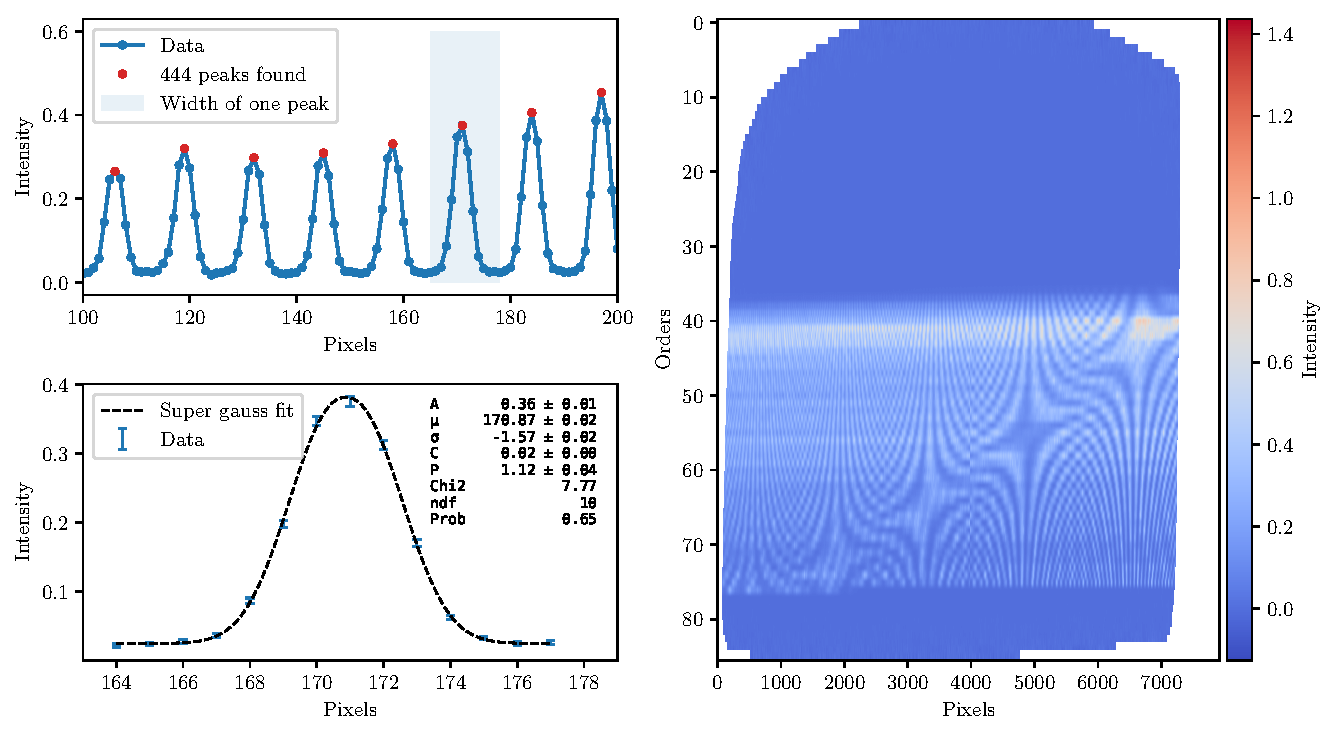
\includegraphics[width=\textwidth]{figures/LFC_peak_fitting_overview.pdf}
            \caption{Right: Measured intensities for the LFC across the CCD (unitless). Upper left: illustration of a few LFC peaks in order 65. Peaks are identified with scipy peak finder. Lower left: each peak is fitted with a super gauss to find the exact top of the peak with uncertainties.}
            \label{fig:LFC_CCD}
        \end{wide}
    \end{SCfigure}

    The LFC generates a series of equadistant (evenly spaced) spectral lines, typically 20,000 lines across 50 orders. The range of the LFC is thus shorter, and for this reason the ThAr exposures can also be used for a rough calibration outside the LFC range. The frequencies of the LFC peaks are given by the relation
    
    \begin{equation}
        \label{eq:LFC_freq_eq}
        v_{n}=v_{\text{rep}} \times n+v_{\text{offset}}
    \end{equation}

    for integers $n$. The repetition rate $v_{\text {rep }}$ and offset frequency $v_{\text {offset }}$ are referenced against a GPS-disciplined quartz oscillator, providing calibration stability corresponding to a fractional uncertainty of less than $8 \times 10^{-12}$ for integration times greater than $1 \mathrm{~s}$. (p. 8, \cite{first_RV_from_EXPRES}). The values I have used in the calibration, $v_{\text{rep}} = 14e9$ and $v_{\text{offset}} = 6.19e9$, were provided by Lars Buchhave, but may be outdated. See figure \ref{fig:LFC_CCD} right side for a plot of the intensities measured across the CCD.

    The following procedure is followed to determine the location of the LFC peaks on the CCD: 1) Find peaks using scipy peak finding algorithm 2) make data slices around each peak with the size of the average distance between peaks, 3) using iminuit do a $\chi^2$ minimisation fit to each peak with a super-gauss plus a linear background. See figure \ref{fig:LFC_CCD} left side.

    A super-gauss, defined in eq. (\ref{eq:LFC_super_gauss}), is a regular gaussian but with an extra parameter, here denoted $P$, that allows the top of the gaussian to be flattened. The last two terms here add a linear background and an offset. 
    
    \begin{equation}
        \label{eq:LFC_super_gauss}
        f(x ; A, B, C, P, \mu, \sigma) = A \exp \left(-\left(\frac{\left(x-\mu\right)^{2}}{2 \sigma^{2}}\right)^{P}\right) + B(x-\mu) + C
    \end{equation}

    The fit then is a minimisation of  

    \begin{equation}
        \label{eq:chi2_super_gauss}
        \chi^{2}=\sum_{i=1}^{N}\left[\frac{y_{i}-f(x ; A, B, C, P, \mu, \sigma)}{\sigma_{i}}\right]^{2}
    \end{equation}

    Where $N$ is the number of data points, $x$ is pixel-space, $y_i$ and $\sigma_i$ is the measured photon count and uncertainty respectively. The fit returns the values and uncertainties for the parameters $A, B, C, P, \mu, \sigma$ when the value of $\chi^2$ is minimized.
    
    We are most interested in $\mu$, which gives the position of the LFC peak on the CCD (in pixel-space). With the intial rough wavelength solution dervied from the ThAr lamp (precalculated in the data set that I've used) I can determine what the approximate wavelength of the LFC peak should be. To find the better wavelength solution I then go look up the closest frequency given by eq. \ref{eq:LFC_freq_eq}. And we now have a map of ~20,000 points on the CCD with a good wavelength solution. 
    
    Of course we need to have a wavelength solution for all points on the CCD and to do that I have explored two approaches: polynomial fitting and cubic interpolation.
    
    \subsubsection{Poly-fit calibration}
    Since the LFC peak positions, as seen in the right plot in figure \ref{fig:LFC_CCD}, appear to exhibit a certain periodic behavour, my initial approach to compute a wavelength solution across the whole CCD was to fit the LFC peak positions with a polynomial. Looking at the residuals of fitting the LFC peaks with polynomial of increasing degree revealed smaller and smaller periodic variations, until reaching 5th degree, see figure \ref{fig:LFC_calib_poly_degrees}. 

    \begin{SCfigure}[1][!ht]%
        \begin{wide}  
            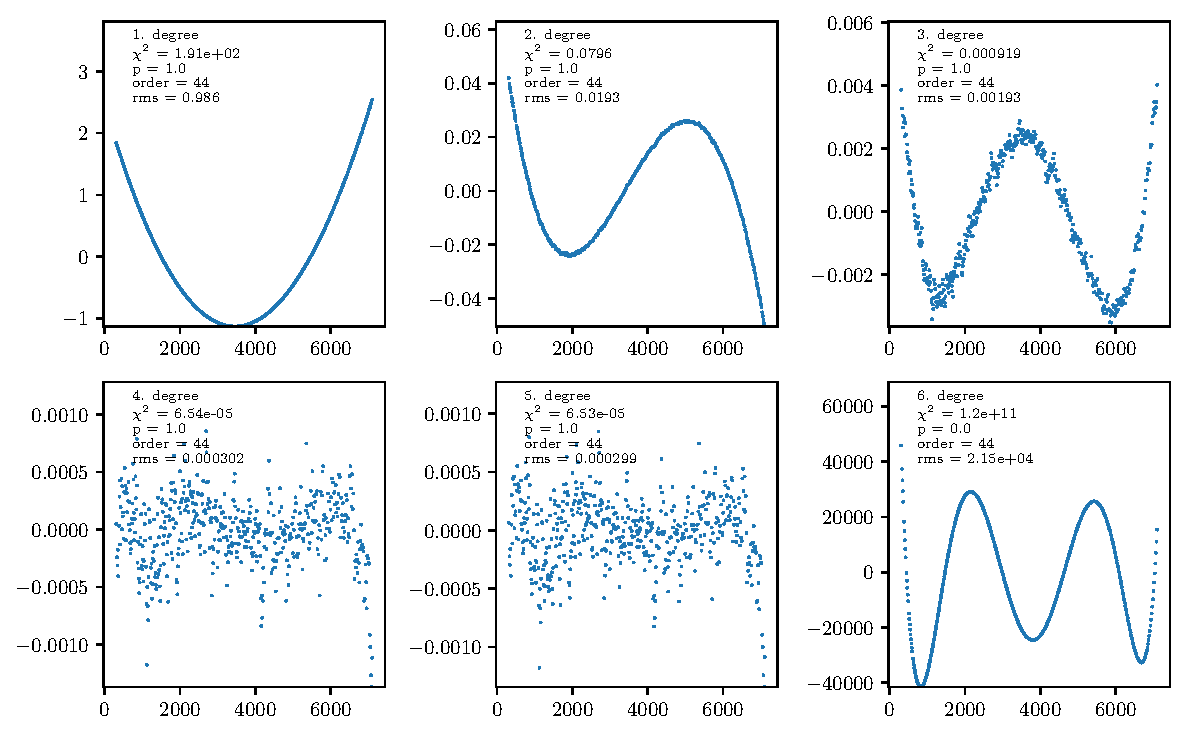
\includegraphics[width=\textwidth]{figures/calib/calib_poly_fit_degrees_order44_residuals_ang.pdf}
            \caption{Residuals from fitting LFC peak positions with polynomials of increasing degree. Pixels on the x-axis and residuals in ångstrom on the y-axis}
            \label{fig:LFC_calib_poly_degrees}
        \end{wide}
    \end{SCfigure}

    But, as the orders are far from idential, this turns out not to work very well across the CCD, see figure \ref{fig:LFC_calib_5th_res}. So I decided to turn to interpolation.

    \begin{SCfigure}[1][!ht]%
        \begin{wide}  
            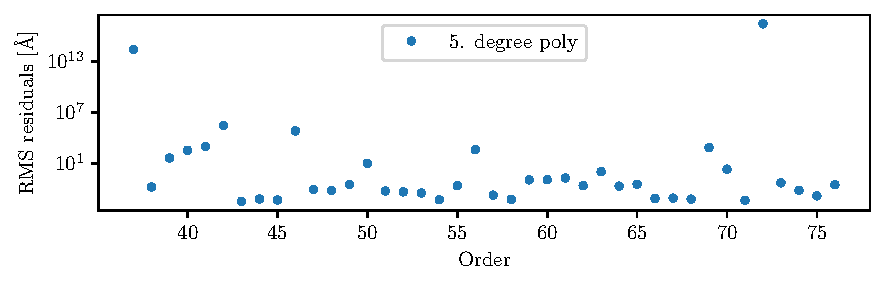
\includegraphics[width=\textwidth]{figures/calib/calib_poly_5th_res.pdf}
            \caption{RMS of residuals from fitting LFC peak positions with 5. degree polynomial. Pixels on the x-axis and residuals in ångstrom on the y-axis}
            \label{fig:LFC_calib_5th_res}
        \end{wide}
    \end{SCfigure}


    \subsubsection{Interpolation calibration}
    A cubic interpolation would force all the residuals to be zero, so in order to evaluate the quality of the method, we can for instance omit every second peak from the interpolation and then compute the residual between the omitted peaks and the resulting interpolation function. We can additionally flip the data set and interpolate the peaks we left out before and compute residuals for the rest, thus ending up with an array of residuals equal to the length of the results from the poly-fit method, allowing us to compare the two, as is done in figure \ref{fig:calib_poly_vs_interp}.

    \begin{SCfigure}[1][!ht]%
        \begin{wide}  
            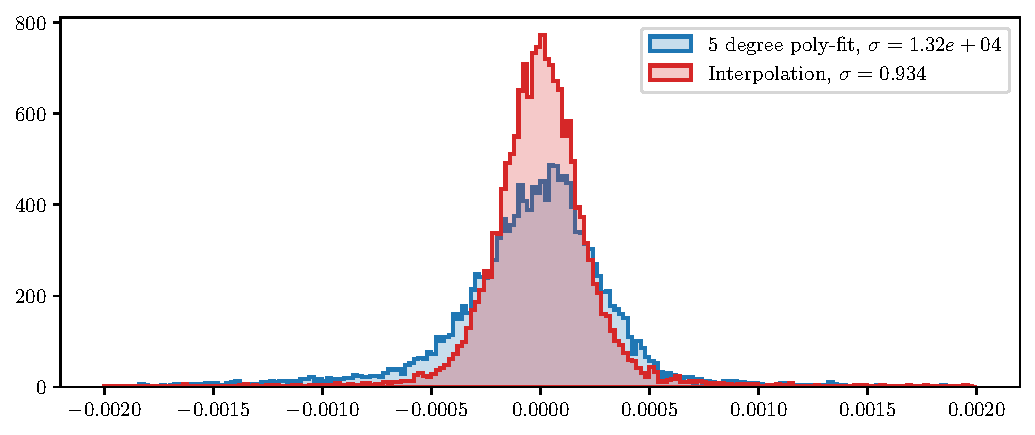
\includegraphics[width=\textwidth]{figures/hist_peak_residuals_poly_and_interp.pdf}
            \caption{Residuals from calibrations performed through a 5th degree poly-fit and a cubic interpolation. Both results contain approximately the same amount of points.}
            \label{fig:calib_poly_vs_interp}
        \end{wide}
    \end{SCfigure}

    The RMS of the residuals from the interpolation come out much smaller than that of the polyfit (values specified in figure \ref{fig:calib_poly_vs_interp}), in this example, suggesting that the interpolation method is superior. It is also worth noting that because the interpolation was done on only half the data points at a time, it will be even better when performed on all data points, as it would be, when used for calibrating data before an RV analysis.

    \vspace{0.5cm}

    \todo{Can we convert this RMS to an RV error ?}

    \todo{add graph comparing residuals using gauss vs super gauss}
    
    \todo{perhaps add plot of changes in parameters across the CCD}




    \subsubsection{Errors in the calibration data}

    The LFC fits files come with an uncertainty on the intensity. It appears however that this uncertainty might be a bit underestimated. We can see this by plotting the $\chi^2$- and P-values for the LFC peak super-gauss fits, as done in figure \ref{fig:calib_errors}. The $\chi^2$ value should be roughly equal to the number of degrees of freedom in the fit (eq. \ref{eq:LFC_super_gauss}), which is: 

    \begin{equation}
        \label{eq:ndof}
        N_\text{dof} = N_\text{data-points} - N_\text{fit-parameters} =  13 - 5 = 8,
    \end{equation}

    as I use about 13 data points in each fit. This is however not the case for the original data (red). Looking at the bottom left plot (red) of the p-values, we can also see that the majority of the fits are very bad. The red chi2 values peak, although only slightly, at around 25, which suggests that the errors are about a factor $\sqrt{3}$ too small (square-root because $\chi^2$ of course is squared and $25/3 \sim 8$). Scaling the errors up by $\sqrt{3}$ yields a chi2 peak at 7.5 and a more flat p-value distribution (green). Scaling by $\sqrt{10}$ is too much (blue). More scale-factors are presented in figure \ref{fig:N_data_points} in appendix \ref{appendix:LFC_errors}. 
                
    \begin{SCfigure}[1][!ht]%
        \begin{wide}  
            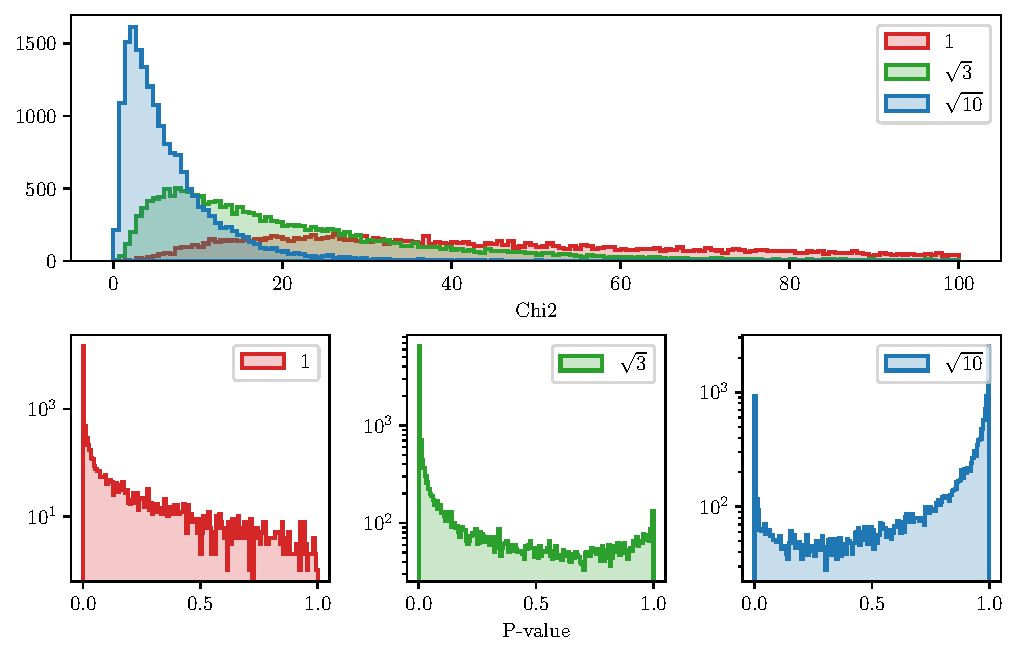
\includegraphics[width=\textwidth]{figures/calib_errors2.pdf}
            \caption{Chi2-values and p-values from individual LFC peak super-gauss fits with photon count (spectrum) errors multiplied by different scale-factors (1, $\sqrt{3}$ and $\sqrt{10}$). See text for more details.}
        \label{fig:calib_errors}
        \end{wide}
    \end{SCfigure}
    
    \bigbreak

    \noindent \textbf{Effects on calibration:} \newline
    The errors used during the production of the calibration residuals shown in figure \ref{fig:calib_poly_vs_interp} I have already multiplied by $\sqrt{3}$. This gave a $\sigma = 0.934$, without this correction I got $\sigma = 2.34$. 

\subsection{RV extraction}

    % To extract radial velocity we need to measure the doppler shift between spectra from different days of observation. The most straight-forward way to do this is to compute the cross-correlation, since, in signal processing in general, the cross-correlation is exactly a measure of the similarity of two data series as a function of the displacement of one relative to the other.

    To extract radial velocities we need to measure the doppler shift between spectra from different days of observation. One way to do that is to compute the cross-correlation, which is a measure of the similarity of two data series as a function of the displacement of one relative to the other.
    
    We can do this either for individual absorption features, chunks of the spectrum a few angstroms wide or entire orders at a time. I've chosen primarily to work with the individual features.

    Due to a lack of access to data consisting of star spectra with associated LFC captures, I've worked on RV extractions using already calibrated data provided by Lily Zhao. This data has been calibrated using a technique called excalibur \cite{zhao2021excalibur}.
    
    The data is visualized in \ref{fig:rv_data_overview}, where the top left shows an extract of wavelength vs. intensity data from an observation of HD 34411. The file also includes a model of the continuum function, with which we can normalize the spectrum through division, shown in the bottom left. On the right side is plotted all continuum normalized data within the EXCALIBUR mask, i.e. data marked as having a proper calibration.

    \begin{SCfigure}[1][!ht]%
        \begin{wide}  
            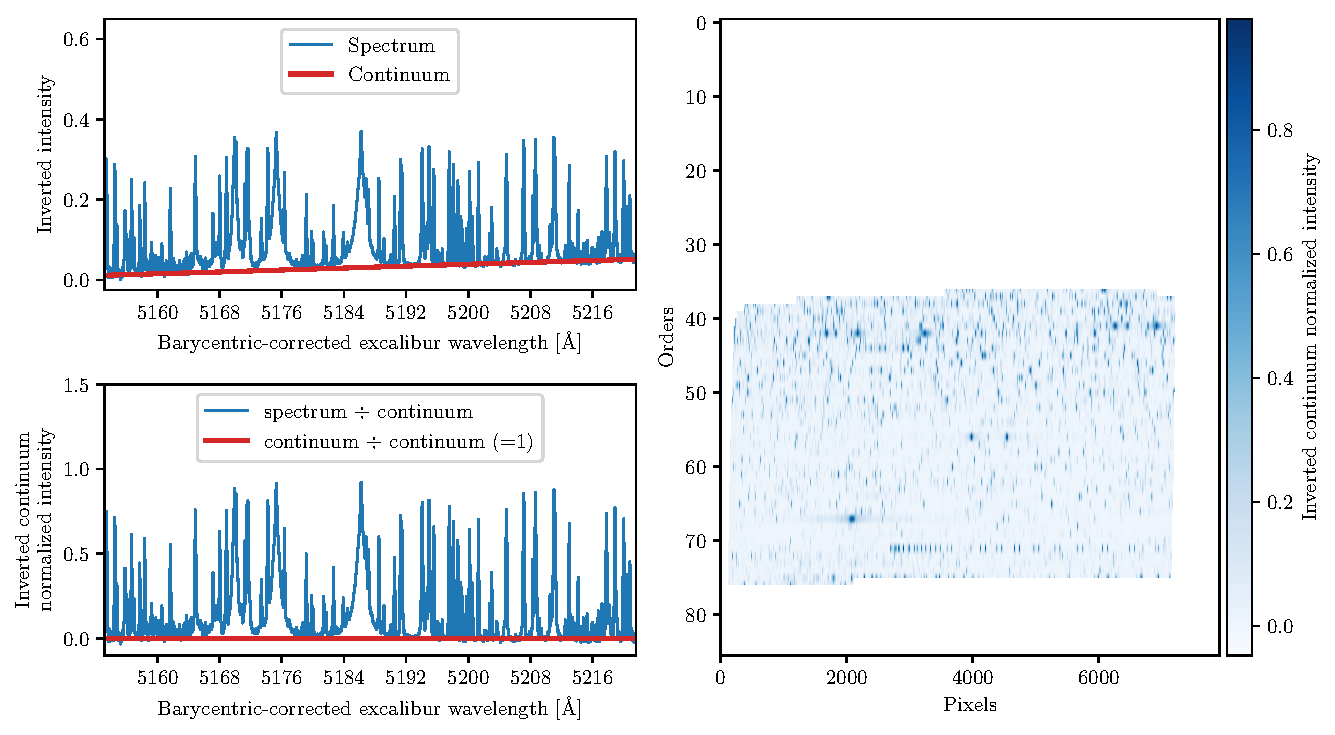
\includegraphics[width=\textwidth]{figures/rv_data_overview.pdf}
            \caption{Overview of excalibur calibrated data from an observation of HD 34411. Upper left: extract of wavelength solution vs. intensity. Lower left: continuum normalized spectrum. Right: all continuum normalized data within the excalibur mask.}
            \label{fig:rv_data_overview}
        \end{wide}
    \end{SCfigure}
            
    \subsubsection{Finding and matching features across observations}

    In order to measure how much individual absorption features move in between observations the first challenge is to find the "same" features in both observations. What follows is a quick rundown of the procedure I've devised:
    
    \begin{itemize}
        \item Load intensities from the data column \verb|"spectrum"| and errors from \verb|"uncertainty"| as well as excalibur calibrated barycentric-corrected wavelengths from \verb|"bary_excalibur"|, all masked by \verb|"excalibur_mask"|.
        \item Normalize intensities and errors with the continuum function from \verb|"continuum"|.
        \item Invert intensities to turn absorption features into positive peaks by $y = 1 - y$.
        \item Locate peaks using \verb|find_peaks| from \verb|scipy.signal| with minimum peak distance of 5 pixels and a minimum peak prominence of 0.25 (unitless).
        \item Finally slice data around each peak with a width of 30 data points. 
    \end{itemize}

    And then to match features/peaks between two observations:

    \begin{itemize}
        \item Iterate through the peaks of observations1 and find the closest peak in observation2. With excalibur calibrated data, peaks should not shift so much that they overlap. However the algorithm laid out so far does sometime match peaks that are far apart or do not resemble each other in shape at all. To bypass such matches we can add two filters:
        \begin{itemize}
            \item Maximum peak distance: We could filter out all matches where the distance between the peaks is equivalant to a radial velocity greater then 12.5 m/s (the RV Jupiter induces in the Sun). However, since we are dealing with discrete data, the difference sometimes comes out much larger than it actually is and a narrow cut of 12.5 m/s would remove many good matches. Instead setting a very generous cut of 0.5 Å, equivalant to about 20-30 km/s depending on the wavelength, filters out the few very bad matches, but leaves the rest.
            
            \item Maximum difference between the area under the graph of two peaks: i.e. the sum of the intensity values. Peaks with similar shapes will give a low difference. Some bad matches can be avoided with this filter, but it also excludes a lot of good matches. Ideally I would keep the filter as strict as possible while maintaining a generous amount of matches. In figure \ref{fig:max_area_diff_vs_n_matches} is plotted the number of matches found between all files as a function of the maximum area difference. From that I conclude that 0.2 is a good option, as the number of matches doesn't rise much with a looser restriction.
        \end{itemize}
    \end{itemize}

    \begin{SCfigure}[1][!ht]%
        \begin{wide}  
            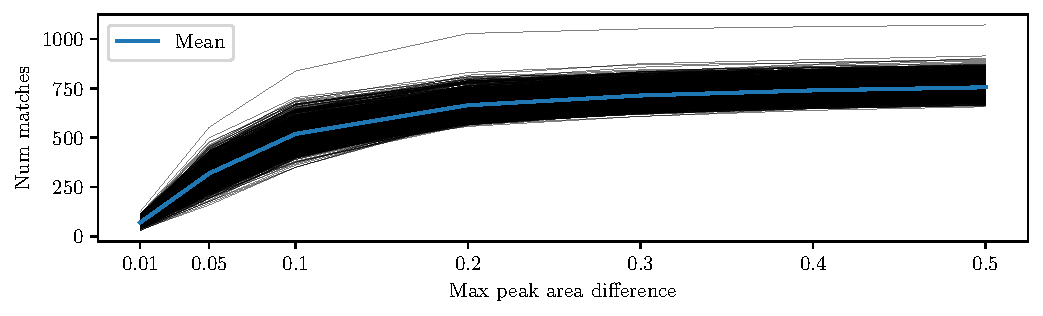
\includegraphics[width=\textwidth]{figures/max_peak_area_diff_vs_Nmatches.pdf}
            \caption{Average number of matches found as a function of max peak area difference for all features in observations for HD 34411.}
            \label{fig:max_area_diff_vs_n_matches}
        \end{wide}
    \end{SCfigure}

    \subsubsection{Cross correlation}

    At this point, I have a list of matching features in different observations. The cross-correlations will be performed as a chi2 minimization fit to find the radial velocity that for each match correctly shifts one feature onto the other one.
    
    Before moving on though, we have to cubic-spline interpolate the spectra data. I do this for two reasons: 1) the shifts we are looking for are much smaller than the individual pixels on the CCD, so we need to be able to shift by sub-pixel amounts, and 2) in order to compute the difference in intensity values between peaks, the intensity values must have the same wavelength solution, but, since EXPRES is calibrated independently for each observation, the wavelength solutions are different.
    
    So I cubic-spline interpolate the spectra data from the first observation in the match, but before interpolating the second observation, I shift the wavelength solution by multiplying the shift factor from equation \ref{eq:our_doppler}. Now I can evaluate the two interpolation functions on a common wavelength range, using $N=1000$ steps\footnote{1000 steps appeared as the best balance between run time and resulting uncertainty. See figure \ref{fig:err_vs_run_time} in appendix \ref{appendix:RV_extraction}}, and I am ready to compute the chi2:
        
    \begin{equation}
        \label{eq:shift_fit_chi2}
        \chi^{2}=\sum_{i=1}^{N}\left[\frac{y_{i}-f(x; v)}{\sigma_{i}}\right]^{2}
    \end{equation}
    
    where $y_i$ are the unshifted interpolated intensity from the first observation, $\sigma_i$ are the errors on the intensity of the first observation also sampled through a cubic-spline interpolation, and the function $f(x; v)$ is the cubic-spline interpolation function given by interpolating the intensity values of the second observation with wavelength values shifted by equation \ref{eq:our_doppler}, evaluated on the wavelength range common to both features: 
    
    \begin{equation}
        f(x; v) = \textbf{interp}[x \times ( 1 + v/c), y]\,(x_\text{common})
    \end{equation}
    
    I then compute the cross-correlation and obtain the radial velocity, $v$, as a minimization of eq (\ref{eq:shift_fit_chi2}) using iminuit.
    
    \todo{Talk about the mean/median etc}

    \subsubsection{Extracting relative shifts from over an overconstrained system}
    
    With the devised method we can now compute the relative readial velocity shift between two observations and get out one number with an uncertainty. The next most obvious step would be to compute the shift between observations 1 and 2, 2 and 3, etc. Doing this however leads to correlated results, as the difference between say observation 1 and 10 will depend on all the observations in bewteen, and if there is one bad one, this will affect all the rest. To circumvent this, we can compute the relative shift bewteen all observations. This will give us an \emph{overconstrained system}, in the sense that there is more information than necessary. All these differences can then be reduced down to a single array, where each shift is relative to all the rest, not only the neighbor. 
    
    Computing the shifts between all observations yields an $N\times N$ upper triangular matrix, where each cell is the shift between observations $i$ and $j$, and thus with a diagonal of zero. I will call this matrix $\Delta V_r^{ij}$, see figure \ref{fig:shift_matrix} for an example.
    
    \begin{SCfigure}[1][!ht]%
        \begin{wide}  
            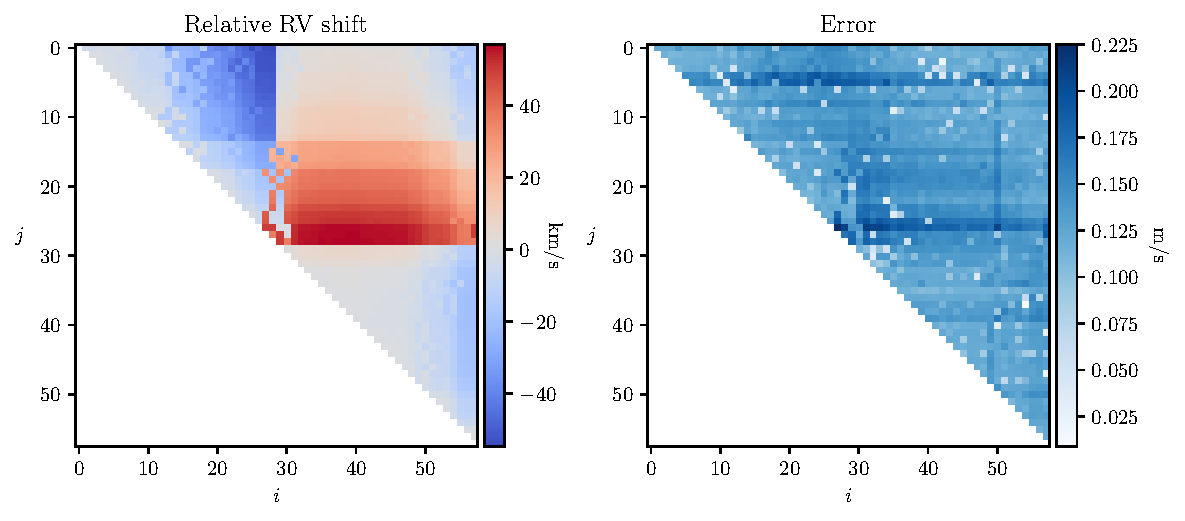
\includegraphics[width=\textwidth]{figures/shfits_matrix_non_bary.pdf}
            \caption{RV shifts matrix computed for HD34411 using non-calibrated, non-barycentric-corrected data (column \texttt{wavelength}). Each cell shows the median relative radial velocity across all features found between observations $i$ and $j$. The diagonal should be zero and has been omitted for the sake of computational speed. I only used one out of the several exposures from each day.}
        \label{fig:shift_matrix}
        \end{wide}
    \end{SCfigure}
            
    To reduce the matrix to one array, we can perform another chi2 minimization fit, defined bellow in equation \ref{eq:matrix_reduction_fit}, in which we fit an array of parameters we can call $V_r^i$ of length $N$ (the number of observations), simply initialized to zero. The chi2 will be at its minimum when it has found an array of velocities $V_r^i$ that best describe all the differences in the matrix $\Delta V_r^{ij}$ and each of the resulting velocities are thus relative not only to its neighbors but to all the other observations as well, thereby avoiding the correlation.
    
    \begin{equation}
        \label{eq:matrix_reduction_fit}
        \chi^{2}=\sum_{i,j = 0}^{N}\left[\frac{ \Delta V_{r}^{ij} - (V_r^i - V_r^j) }{\sigma(\Delta V_{r}^{ij})}\right]^{2} \quad : \quad i < j.
    \end{equation}

    For the sake of illustrating the method, I've analysed non-barycentric corrected data, in which we should be able to see the movement of the Earth around the center of mass of the solar system. That is the data plotted in the matrix in figure \ref{fig:shift_matrix} and the resulting extracted relative radial velocities (the fit parameters $V_r^i$) are plotted in figure \ref{fig:RV_results_non_barycentric} (black), where we see a clear signal of Earth's movement. I've fitted the data with a periodic function and found that the period is $(367.522 \pm 5\mathrm{e}{-5})$ days. Then there are three things to notice: 1) the error does not cover the discrepancy with the acrtual value of 365.24 days, 2) the very high chi2 value, and 3) the p-value of zero. These suggest very clearly that my errors are wrong. Nevertheless, the signal is clear, from which I confirm that my method in general is working. Comparing with the direct differences between observations plotted in blue in figure \ref{fig:RV_results_non_barycentric}, it is also clear that the last step of computing the relative shift between all observatons is vital. 

    \begin{SCfigure}[1][!ht]%
        \begin{wide}  
            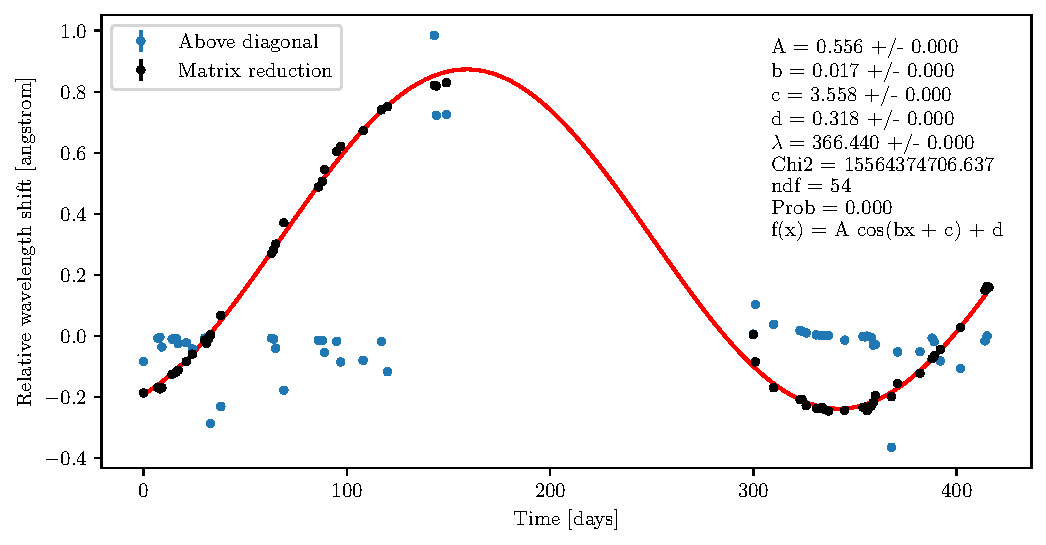
\includegraphics[width=\textwidth]{figures/shift_non_bary_centric.pdf}
            \caption{Computed relative wavelength shifts for HD34411 using non-calibrated, non-barycentric-corrected data (column \texttt{wavelength}). Blue: the shifts from day to day. Black: values computed through the chi2 minimization.}
            \label{fig:RV_results_non_barycentric}
        \end{wide}
    \end{SCfigure}

    \subsubsection{Computational run times}
    \todo{add number of function calls for the fitting}
    \todo{add number of peak analyzed and so on}
    \todo{add run times}



